\section{Experiments and results}
\subsection{Experimental setup}
All experiments  launched  on the new virtual machine which is running on OpenStack\cite{openstack} Platform with following characteristics: 
\begin{table}[ht]
\begin{tabular}{ll}
RAM & 4GB \\
VCPUs & 2 VCPU with 2500 Mhz \\
Disk & 40GB \\
OS &  Ubuntu 16.04.4 LTS\\
\end{tabular}
\end{table}

Tests were conducted with each platform 50 times. As evaluation criterion for demonstrating the test environment, used system tests such as download, start, stop, delete. Since CloudchecR is a web-based platform, it was not tested for these characteristics. Also as a testing function used actions with the provider, in this case, each platform worked with an out-of-order provider on AWS server, with the same region and access keys. All of the platforms tested for creation, listing, deleting provider, also ManageIQ and Cloudcheckr for synchronisation time because of architecture design. The following versions of  platforms used in this experiments:

\begin{table}[ht]
\begin{tabular}{ll}
Mist.io  & Cloud Management Platform version: 2.0 \\
ManageIQ & gaprindashvili-3 \\
CloudcheckR & last update May 21, 2018 \\
Apache Libcloud & version 2.3.0\\
\end{tabular}
\end{table}

For the set of the experiments used one single matrix file, which together with raw and aggregated data, can be found along with the source code for this link(put public link).

\subsection{Results}
Architecture of the testbed was designed in that way that overhead is minimal and can be can be neglected.
All the information which given below, such as graphics and tables in the latex format, were generated by the test platform itself. In this part, there will be no in-depth analysis of the data, since comparing different types of platforms is not relevant. The purpose of this work is to provide an approach to creating a test platform for multi-cloud management platforms.

Table \ref{tab:time} shows the results of time evaluation from which concluded that liblcoud performs the fastest system operations since it is an uncomplicated library and it is much simpler than other platforms. Mistio is a multi-image docker platform and because of this loses ManageIQ in the boot time, but shows better results t in time of start and stop the system.

\begin{table}[ht]
\caption{Time criteria exemplary}
\begin{center}
\begin{tabular}{lllllll}
	\hline
	 \multirow{3}{*}{src} & \multirow{3}{*}{action} & \multirow{3}{*}{platform} & \multicolumn{3}{c}{metrics} \\ 
	& & & \multicolumn{3}{c}{time}\\ 
 	& & & mu & sigma & median\\ 
 	\hline
 \\[-1em] \multirow{12}{*}{\rotatebox[origin=c]{90}{*-system}} & \multirow{3}{*}{download} & manageiq & 1.06e+05 & 1.32e+05 & 8.21e+04\\ \\[-1em] 
 	 & & libcloud & 1717.40 & 120.34 & 1711.85\\ \\[-1em] 
 	 & & mistio & 4.25e+05 & 7.21e+05 & 2.58e+05\\ \\[-1em] 
 	\\[-1em] \cline{2-6} \\[-1em] & \multirow{3}{*}{start} & manageiq & 2.00e+05 & 2455.44 & 1.99e+05\\ \\[-1em] 
 	 & & libcloud & 3430.90 & 218.90 & 3445.10\\ \\[-1em] 
 	 & & mistio & 7.93e+04 & 2927.29 & 7.86e+04\\ \\[-1em] 
 	\\[-1em] \cline{2-6} \\[-1em] & \multirow{3}{*}{stop} & manageiq & 654.38 & 92.43 & 645.32\\ \\[-1em] 
 	 & & libcloud & 1575.64 & 125.65 & 1580.09\\ \\[-1em] 
 	 & & mistio & 1.84e+04 & 483.24 & 1.83e+04\\ \\[-1em] 
 	\\[-1em] \cline{2-6} \\[-1em]  & \multirow{3}{*}{remove} & manageiq & 3670.05 & 185.47 & 3669.37\\ \\[-1em] 
 	 & & libcloud & 1.99 & 1.89 & 1.45\\ \\[-1em] 
 	 & & mistio & 6.28e+04 & 7756.02 & 6.08e+04\\ \\[-1em] 
 	 \\[-1em] \hline
	\multirow{14}{*}{\rotatebox[origin=c]{90}{aws-provider}} & \multirow{4}{*}{create} & cloudcheckr & 2411.50 & 263.09 & 2339.36\\ \\[-1em] 
 	 & & manageiq & 254.98 & 140.68 & 225.29\\ \\[-1em] 
 	 & & libcloud & 781.10 & 109.80 & 732.14\\ \\[-1em] 
 	 & & mistio & 1363.78 & 270.84 & 1339.77\\ \\[-1em] 
 	\\[-1em] \cline{2-6} \\[-1em] & \multirow{4}{*}{list} & cloudcheckr & 993.05 & 126.11 & 953.57\\ \\[-1em] 
 	 & & manageiq & 200.26 & 48.64 & 187.33\\ \\[-1em] 
 	 & & libcloud & 338.55 & 38.84 & 328.69\\ \\[-1em] 
 	 & & mistio & 20.77 & 10.16 & 17.31\\ \\[-1em] 
 	\\[-1em] \cline{2-6} \\[-1em] & \multirow{2}{*}{sync} & cloudcheckr & 4.25e+05 & 6.15e+04 & 4.21e+05\\ \\[-1em] 
 	 & & manageiq & 6.94e+05 & 2.06e+06 & 2.75e+04\\ \\[-1em] 
 	\\[-1em] \cline{2-6} \\[-1em] & \multirow{4}{*}{delete} & cloudcheckr & 1063.39 & 192.29 & 1000.20\\ \\[-1em] 
 	 & & manageiq & 7482.43 & 3131.54 & 7014.02\\ \\[-1em] 
 	 & & libcloud & 0.01 & 0.01 & 0.01\\ \\[-1em] 
 	 & & mistio & 103.77 & 41.60 & 88.88\\ \\[-1em] 
 	\\[-1em] \hline
\end{tabular}
\end{center}
\label{tab:time}
\end{table}

In the results of provider operations, liblcoud was again the fastest, from the graphical interface platforms, good results were also shown by the Mistio, unlike ManageIQ and CloudcheckR, there is no need for synchronisation time. At the same time, the creation of the provider the fastest results shown by the ManagqIQ platform that can be seen in figure \ref{creti}.

\begin{figure}[htbp]
\centerline{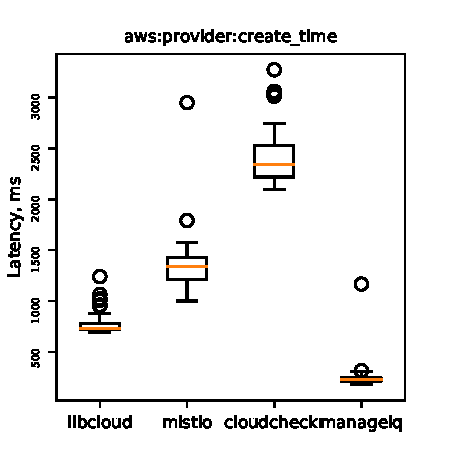
\includegraphics[scale=1]{pics/provider_create_time.pdf}}
\caption{Creation time of provider}
\label{creti}
\end{figure}

Table \ref{tab:cpu} and \ref{tab:mem} show the characteristics of the CPU time and Memory KB
from both results it follows that in docker-base platforms the results are not so stable as seen in figure \ref{crecpu}, but it explained by the fact that the systems are complex and they load themselves, while the operations that were carried out were simple and not resource-intensive, which can be seen from the libcloud on figure \ref{libaws}, were the platform itself is not super resource consumption.
\begin{figure}[htbp]
\centerline{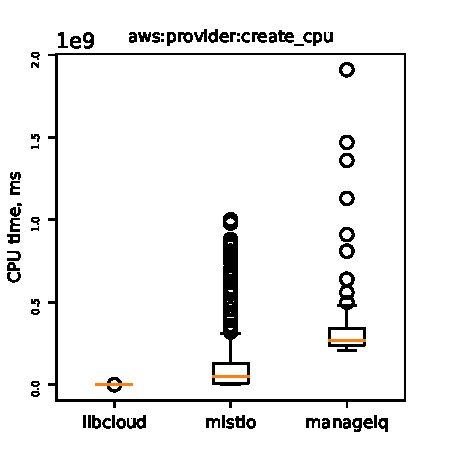
\includegraphics[scale=1]{pics/provider_create_cpu.pdf}}
\caption{Creation CPU time of provider}
\label{crecpu}
\end{figure}

\begin{figure}[htbp]
\centerline{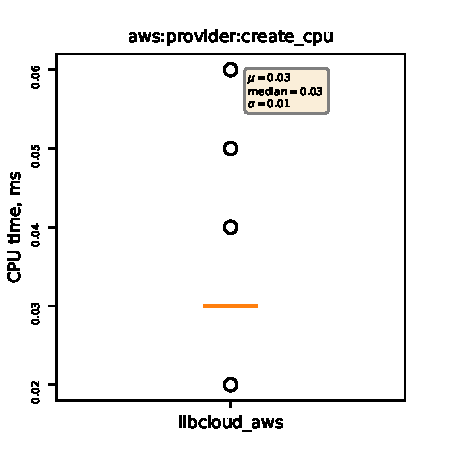
\includegraphics[scale=1]{pics/libcloud_aws.pdf}}
\caption{Creation time of provider}
\label{libaws}
\end{figure}

\begin{table}[ht]
\caption{Creation CPU time of provider for libcloud}
\begin{center}
\begin{tabular}{lllllll}
	\hline
	\multirow{3}{*}{src} & \multirow{3}{*}{action} & \multirow{3}{*}{platform} & \multicolumn{3}{c}{metrics} \\ 
	& & & \multicolumn{3}{c}{cpu}\\ 
 	& & & mu & sigma & median\\ 
 	\hline
 \\[-1em] \multirow{10}{*}{\rotatebox[origin=c]{90}{aws-provider}} & \multirow{3}{*}{create} & manageiq & 4.24e+08 & 3.67e+08 & 2.70e+08\\ \\[-1em] 
 	 & & libcloud & 0.03 & 0.01 & 0.03\\ \\[-1em] 
 	 & & mistio & 1.12e+08 & 1.74e+08 & 5.00e+07\\ \\[-1em] 
 	\\[-1em] \cline{2-6} \\[-1em] & \multirow{3}{*}{list} & manageiq & 5.88e+08 & 3.60e+08 & 4.40e+08\\ \\[-1em] 
 	 & & libcloud & 0.01 & 0.01 & 0.01\\ \\[-1em] 
 	 & & mistio & 9.34e+07 & 1.79e+08 & 3.00e+07\\ \\[-1em] 
 	\\[-1em] \cline{2-6} \\[-1em]  & \multirow{1}{*}{sync} & manageiq & 6.58e+11 & 1.93e+12 & 3.37e+10\\ \\[-1em] 
 	\\[-1em] \cline{2-6} \\[-1em]  & \multirow{3}{*}{delete} & manageiq & 7.62e+09 & 5.42e+09 & 6.36e+09\\ \\[-1em] 
 	 & & libcloud & 0.00 & 0.00 & 0.00\\ \\[-1em] 
 	 & & mistio & 9.30e+07 & 1.52e+08 & 4.00e+07\\ \\[-1em] 
 	\\[-1em] \hline
\end{tabular}
\end{center}
\label{tab:cpu}
\end{table}

\begin{table}[ht]
\caption{Memory KB criteria evaluation}
\begin{center}
\begin{tabular}{lllllll}
	\hline
	\multirow{3}{*}{src} & \multirow{3}{*}{action} & \multirow{3}{*}{platform} & \multicolumn{3}{c}{metrics} \\ 
	& & & \multicolumn{3}{c}{memory}\\ 
 	& & & mu & sigma & median\\ 
 	\hline
 \\[-1em] \multirow{10}{*}{\rotatebox[origin=c]{90}{aws-provider}} & \multirow{3}{*}{create} & manageiq & -1.40e+07 & 7.38e+07 & 7.37e+04\\ \\[-1em] 
 	 & & libcloud & 2.73e+05 & 4.31e+05 & 0.00\\ \\[-1em] 
 	 & & mistio & 4.04e+05 & 5.46e+06 & 0.00\\ \\[-1em] 
 	\\[-1em] \cline{2-6} \\[-1em] & \multirow{3}{*}{list} & manageiq & 2.82e+06 & 1.56e+07 & 1.68e+05\\ \\[-1em] 
 	 & & libcloud & 1.11e+04 & 4.64e+04 & 0.00\\ \\[-1em] 
 	 & & mistio & 3.08e+04 & 6.05e+06 & 0.00\\ \\[-1em] 
 	\\[-1em] \cline{2-6} \\[-1em] & \multirow{1}{*}{sync} & manageiq & 2.00e+08 & 9.66e+07 & 1.75e+08\\ \\[-1em] 
 	\\[-1em] \cline{2-6} \\[-1em] & \multirow{3}{*}{delete} & manageiq & -1.63e+08 & 7.67e+07 & -1.76e+08\\ \\[-1em] 
 	 & & libcloud & 0.00 & 0.00 & 0.00\\ \\[-1em] 
 	 & & mistio & -1.47e+05 & 6.56e+06 & 0.00\\ \\[-1em] 
 	\\[-1em] \hline
\end{tabular}
\end{center}
\label{tab:mem}
\end{table}

